\documentclass[smallextended]{svjour3}
\usepackage[]{graphicx}\usepackage[]{color}
% maxwidth is the original width if it is less than linewidth
% otherwise use linewidth (to make sure the graphics do not exceed the margin)
\makeatletter
\def\maxwidth{ %
  \ifdim\Gin@nat@width>\linewidth
    \linewidth
  \else
    \Gin@nat@width
  \fi
}
\makeatother

\definecolor{fgcolor}{rgb}{0.345, 0.345, 0.345}
\makeatletter
\@ifundefined{AddToHook}{}{\AddToHook{package/xcolor/after}{\definecolor{fgcolor}{rgb}{0.345, 0.345, 0.345}}}
\makeatother
\newcommand{\hlnum}[1]{\textcolor[rgb]{0.686,0.059,0.569}{#1}}%
\newcommand{\hlstr}[1]{\textcolor[rgb]{0.192,0.494,0.8}{#1}}%
\newcommand{\hlcom}[1]{\textcolor[rgb]{0.678,0.584,0.686}{\textit{#1}}}%
\newcommand{\hlopt}[1]{\textcolor[rgb]{0,0,0}{#1}}%
\newcommand{\hlstd}[1]{\textcolor[rgb]{0.345,0.345,0.345}{#1}}%
\newcommand{\hlkwa}[1]{\textcolor[rgb]{0.161,0.373,0.58}{\textbf{#1}}}%
\newcommand{\hlkwb}[1]{\textcolor[rgb]{0.69,0.353,0.396}{#1}}%
\newcommand{\hlkwc}[1]{\textcolor[rgb]{0.333,0.667,0.333}{#1}}%
\newcommand{\hlkwd}[1]{\textcolor[rgb]{0.737,0.353,0.396}{\textbf{#1}}}%
\let\hlipl\hlkwb

\usepackage{framed}
\makeatletter
\newenvironment{kframe}{%
 \def\at@end@of@kframe{}%
 \ifinner\ifhmode%
  \def\at@end@of@kframe{\end{minipage}}%
  \begin{minipage}{\columnwidth}%
 \fi\fi%
 \def\FrameCommand##1{\hskip\@totalleftmargin \hskip-\fboxsep
 \colorbox{shadecolor}{##1}\hskip-\fboxsep
     % There is no \\@totalrightmargin, so:
     \hskip-\linewidth \hskip-\@totalleftmargin \hskip\columnwidth}%
 \MakeFramed {\advance\hsize-\width
   \@totalleftmargin\z@ \linewidth\hsize
   \@setminipage}}%
 {\par\unskip\endMakeFramed%
 \at@end@of@kframe}
\makeatother

\definecolor{shadecolor}{rgb}{.97, .97, .97}
\definecolor{messagecolor}{rgb}{0, 0, 0}
\definecolor{warningcolor}{rgb}{1, 0, 1}
\definecolor{errorcolor}{rgb}{1, 0, 0}
\makeatletter
\@ifundefined{AddToHook}{}{\AddToHook{package/xcolor/after}{
\definecolor{shadecolor}{rgb}{.97, .97, .97}
\definecolor{messagecolor}{rgb}{0, 0, 0}
\definecolor{warningcolor}{rgb}{1, 0, 1}
\definecolor{errorcolor}{rgb}{1, 0, 0}
}}
\makeatother
\newenvironment{knitrout}{}{} % an empty environment to be redefined in TeX

\usepackage{alltt}
\newcommand{\SweaveOpts}[1]{}  % do not interfere with LaTeX
\newcommand{\SweaveInput}[1]{} % because they are not real TeX commands
\newcommand{\Sexpr}[1]{}       % will only be parsed by R

    
\smartqed  % flush right qed marks, e.g. at end of proof

\usepackage[colorlinks=true,linkcolor={blue},citecolor={blue},urlcolor={blue}]{hyperref}
%\usepackage{caption}
% Add longtable and ctable packages
\usepackage{longtable,ctable}
\usepackage{amsmath}
\usepackage{amssymb}
\usepackage{amsfonts}
\usepackage{multirow}
%\usepackage{amsthm}
\usepackage{graphicx}

\usepackage{booktabs}
%\usepackage{bookmark}

%\usepackage{caption}
%\usepackage{capt-of}

\usepackage{amsmath}
\usepackage{graphicx}
\usepackage{mathptmx}
\usepackage{natbib}

\usepackage{setspace}

%\usepackage{tikz-feynman}
%\usepackage{tikz} 
%\usetikzlibrary{positioning}
\usepackage[utf8]{inputenc}
\usepackage{pgf}


\usepackage{algorithm}
\usepackage{algpseudocode}
\usepackage{enumerate}


\raggedbottom

%\def\convp{\stackrel{p}\rightarrow}
%\def\barn{\bar{N}}
%\def\bary{\bar{Y}}
%\def\baryj{\bar{Y}_{j}(s)}

%\def\barnt{\bar{N}(t)}
%\def\baryjt{\bar{Y}_{j}(t)}
%\def\baryat{\bar{Y}_{0}(t)}
%\def\barybt{\bar{Y}_{1}(t)}
%\def\barnjt{\bar{N}_{j}(t)}
%\def\barnat{\bar{N}_{0}(t)}
%\def\barnbt{\bar{N}_{1}(t)}
%\def\barajt{\bar{A}_{j}(t)}
%\def\baraat{\bar{A}_{0}(t)}
%\def\barabt{\bar{A}_{1}(t)}


% WLR definitions
\def\Grg{\hbox{G}^{\rho,\gamma}}
\newcommand{\fh}[2]{\ensuremath{\hbox{FH}({{#1},{#2}})}}
\newcommand{\Zfh}[2]{\ensuremath{\hbox{Z}^{{#1},{#2}}}}
\def\Zrg{\hbox{Z}^{\rho,\gamma}}
\newcommand{\lam}[2]{\ensuremath{\lambda^{h}(#1|#2)}}
\newcommand{\barF}[2]{\ensuremath{\bar{F}(#1|#2)}}
\newcommand{\barG}[2]{\ensuremath{\bar{G}(#1|#2)}}

%\def\barGt{\bar{G}(t)}
%\def\Fone{\bar{F}_{1}(t)}
%\def\Fzero{\bar{F}_{0}(t)}

%\def\hatFjt{\hat{\bar{F}}_{j}(t)}
%\def\hatFjs{\hat{\bar{F}}_{j}(s)}
%\def\Fjt{\bar{F}_{j}(t)}

%\def\Zmax{Z_{max}}
%\def\Zmaxstar{Z^{\dagger}_{max}}
%\def\zmax{z_{max}}

%\def\bmax{\hat\beta_{max}}
%\def\bw{\hat\beta_{w}}
%\def\bwstar{\beta_{w}^{*}}

\def\sumin{\sum_{i=1}^n}
\def\nsumin{n^{-1}\sum_{i=1}^n}

\def\ns{n_{0}+n_{1}}
\def\na{n_{0}}
\def\nb{n_{1}}

\newcommand{\indep}{\perp \!\!\! \perp}


\textheight=9.0in \textwidth=6.0in 
\topmargin=0in
\evensidemargin=0in \oddsidemargin=0in




\begin{document}




















\begin{table}

\caption{\label{tab:unnamed-chunk-5}\label{tab:simex1} Simulated example Cox hazard ratio (hr) estimates (denoted $\hat\theta$) for the ITT population and subgroups $H$ and $H^{c}$.
$\hat\theta(ITT)$ denotes the overall ITT population hr estimate and $\hat\theta(H)$ denotes the hr estimate based on the a-priori known (true) $H$ subgroup
$\hat\theta(\hat{H})$ denotes the hr estimate based on the estimated subgroup H and $\hat\theta^{*}(\hat{H})$ denotes the corresponding bootstrap bias-corrected estimate.  
Estimates for the complement $H^{c}$ are defined analogously.}
\centering
\begin{tabular}[t]{lccccc}
\toprule
  & HR Estimate & Lower & Upper & C(a-priori) & C(fixed)\\
\midrule
\addlinespace[0.3em]
\multicolumn{6}{l}{\textbf{ITT}}\\
\hspace{1em}ITT & 0.8376815 & 0.6873089 & 1.020953 & . & .\\
\addlinespace[0.3em]
\multicolumn{6}{l}{\textbf{H subgroup estimates}}\\
\hspace{1em}H a-priori & 2.35787 & 1.47058 & 3.780517 & . & 1\\
\hspace{1em}H estimate & 3.077133 & 1.604064 & 5.902971 & 1 & 1\\
\hspace{1em}Bias-corrected H estimate & 2.233123 & 1.456923 & 3.422858 & 1 & 1\\
\addlinespace[0.3em]
\multicolumn{6}{l}{\textbf{H-complement subgroup estimates}}\\
\hspace{1em}$H^{c}$ a-priori & 0.6721508 & 0.5372828 & 0.8408731 & . & 1\\
\hspace{1em}$H^{c}$ estimate & 0.7330196 & 0.5924729 & 0.9069068 & 1 & 1\\
\hspace{1em}Bias-corrected $H^{c}$ estimate & 0.7438026 & 0.5929508 & 0.9330324 & 1 & 1\\
\bottomrule
\end{tabular}
\end{table}





As an illustration we consider a simulated dataset generated as described in Section 3 below.   In this simulated example there are 
$n=700$ subjects, randomized 1:1, where the underlying (marginal) hazard ratio for the harm population $H$ is $2.5$, and for the complement $H^{c}$, the (marginal) hazard ratio is $0.65$.  The overall (marginal) hazard ratio 
is $0.71$.  Here the actual number of subjects in the $H$ subgroup is 
$101$ and the number of subjects in the complement equals $599$.  

Applying our novel procedure the 
estimated subgroup $\hat{H}$ consists of $64$ subjects and thus 
$636$ in the estimated complement $\hat{H}^{c}$. The number of subjects in $H$ that are included in $\hat{H}$ is $52$ (i.e., $|H \cap \hat{H}|=52$): Of the $101$ subjects in $H$, 
$52/101=51\%$ are correctly classified and of the $64$ subjects in $\hat{H}$, $52/64=81\%$ are correctly classified.  For the complement, the number of subjects in $H^{c}$ that are included in $\hat{H}^{c}$ is $587$: Of the $599$ subjects in $H^{c}$, 
$587/599=98\%$ are correctly classified and of the $636$ subjects in $\hat{H}^{c}$, $587/636=92\%$ are correctly classified.



\begin{figure}[h!]
\begin{center}
\begin{knitrout}
\definecolor{shadecolor}{rgb}{0.969, 0.969, 0.969}\color{fgcolor}
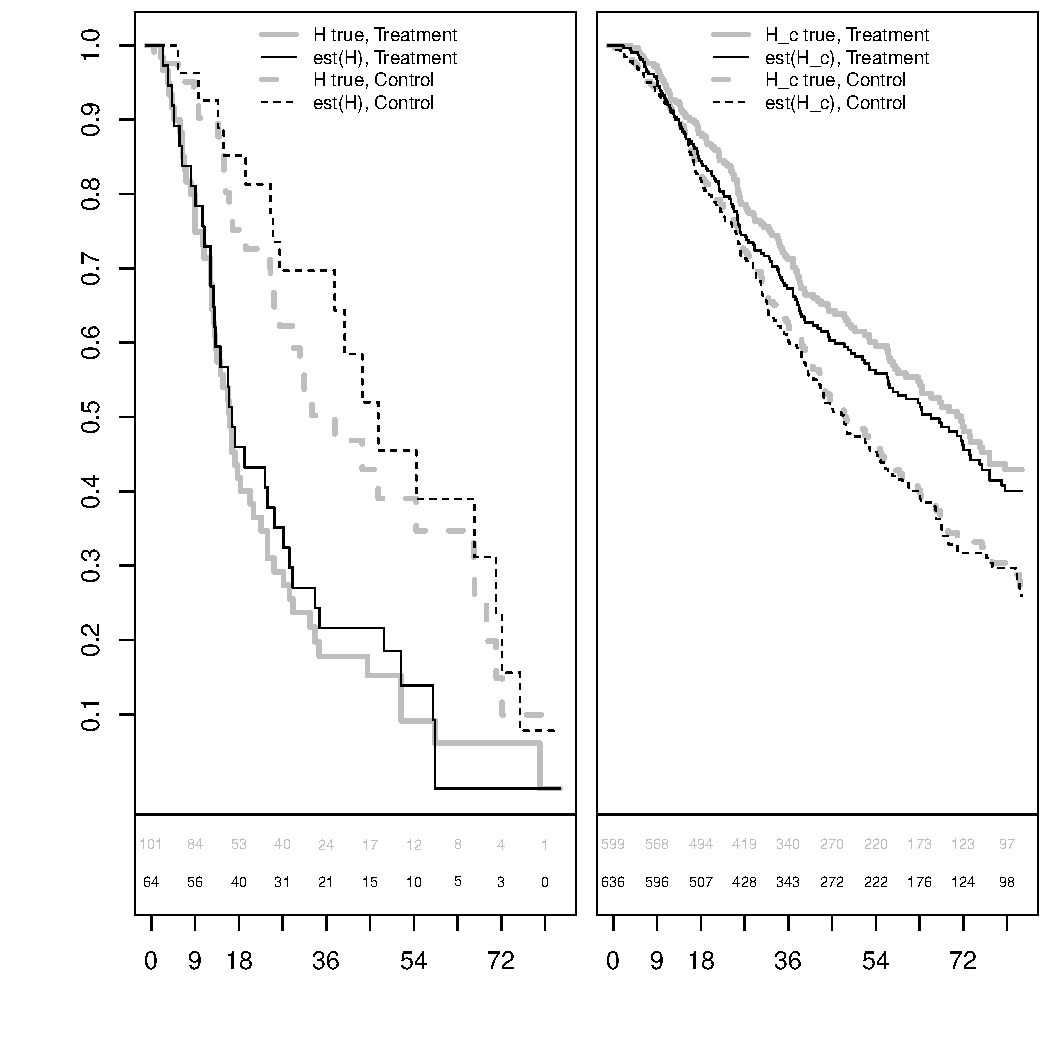
\includegraphics[width=400px,height=250px]{figure/sim_ex1-1} 
\end{knitrout}
\end{center}
\caption{Simulated example}\label{fig:simex1}
\end{figure}







\bibliographystyle{spbasic}      % basic style, author-year citations
\bibliography{../../subgroups_ref}
\end{document}
